\documentclass[spanish]{article}
\usepackage[utf8]{inputenc}
\usepackage{amsmath}
\usepackage{listings}
\usepackage{xcolor}
\usepackage{geometry}
\usepackage{graphicx} 
\usepackage{pdfpages}
\usepackage{listings}
\usepackage{xcolor}
\usepackage{titling}
\usepackage{array}
\usepackage{tabularx}
\usepackage{booktabs}
\usepackage{float}
\usepackage[es-tabla]{babel}
 \usepackage[normalem]{ulem}
  \useunder{\uline}{\ul}{}
\usepackage{amsmath}
\usepackage{hyperref}
\usepackage{cleveref}

\geometry{a4paper, margin=1in}
\crefname{tabla}{\spanishtablename}{\spanishtablename}
\setlength{\parskip}{1em}

\lstset{
    basicstyle=\ttfamily\small,
    breaklines=true,
    columns=fullflexible,
    frame=single,
    backgroundcolor=\color{gray!10},
    keywordstyle=\color{blue},
    commentstyle=\color{olive},
    stringstyle=\color{magenta},
    showstringspaces=false
}


\renewcommand{\contentsname}{Contenido}
\begin{document}
	\begin{titlepage}
		\centering
		%{\bfseries\LARGE Universidad Autónoma de Madrid \par}
		\vspace{4cm}
		{\scshape\Large Herramientas de Programación en Bioinformática y Biología Computacional \par}
		\vspace{6cm}
		{\scshape\Huge Proyecto de Base de Datos de Pruebas Hospitalarias \par}
		%\vspace{3cm}
		\vfill
		{\Large Autoras: \par}
		{\Large Deyanira Borroto Alburquerque\\
        		Tania Gonzalo Santana \par}
		\vfill
		{\Large Noviembre 2024 \par}
		{\scshape\normalsize Universidad Autónoma de Madrid \par}
\end{titlepage}


% Página 2: Índice
\tableofcontents


\newpage % Salto de página para continuar con el contenido

\section{Introducción al problema a resolver}
% Describir aquí el problema que la base de datos está destinada a resolver.

\subsection{Contexto}

En el ámbito de la salud, la gestión eficiente y precisa de la información es crucial para garantizar la calidad de la atención médica. Los hospitales y centros de salud realizan una gran cantidad de pruebas diagnósticas diariamente, generando un volumen significativo de datos difíciles de manejar que deben ser gestionados de manera efectiva. Esta información relacionada con las pruebas hospitalarias incluye datos de pacientes, médicos, pruebas, muestras obtenidas, resultados y facturación, entre otros.

La digitalización de los registros médicos ha transformado la manera en que se maneja toda esta información en el sector salud. Sin embargo, muchos sistemas aún enfrentan desafíos significativos en términos de integración, accesibilidad y precisión de los datos. Esto puede llevar a errores en el diagnóstico y retrasos en el tratamiento, afectando esto a la salud y supervivencia de los pacientes.

El diseño y desarrollo de una base de datos relacional para la gestión de pruebas hospitalarias ofrece múltiples beneficios: mejora en la precisión de los datos, eficiencia operativa, seguridad y privacidad de los datos de los pacientes y facilidad de acceso, entre otras. Por ejemplo, una base de datos relacional de este tipo permitiría reducir los errores humanos al automatizar la entrada y manejo de datos, asegurando que información crítica como pueden ser resultados de las pruebas y los datos de los pacientes sea precisa y actualizada. 

Puesto que la implementación de una base de datos relacional para la gestión de pruebas hospitalarias no solo optimiza la administración de la información, sino que también contribuye a mejorar la calidad de la atención médica, la seguridad del paciente y la eficiencia operativa del centro de salud. Este proyecto busca desarrollar un sistema que aborde estos desafíos y proporcione una solución integral para la gestión de pruebas hospitalarias.

\subsection{Objetivo}

El objetivo principal de este proyecto es diseñar y desarrollar un modelo de base de datos relacional para gestionar los registros de pruebas hospitalarias. Esto incluye organizar y almacenar información de pacientes, médicos, pruebas, muestras, resultados y facturas de una manera que garantice la integridad de los datos y una recuperación eficiente.

\subsection{Alcance}

Este proyecto cubrirá la gestión de pacientes, médicos, pruebas, muestras, resultados y facturas, asegurando que todos los datos estén correctamente estructurados y relacionados.

\newpage
\section{Diagrama de Entidad-Relación (ER)}
Una vez identificado el problema a resolver, debemos modelarlo mediante un diagrama Entidad-Relación (ER). A continuación se indican los pasos a seguidos para la obtención del digrama ER de nuestra base de datos a la se le ha denominado "Base de Datos de Pruebas Hospitalarias".

\subsection{Identificación de entidades y atributos}
El primer paso en la creación del diagrama ER es identificar las entidades, los atributos y las relaciones entre ellas. En este caso, hemos definido seis entidades: paciente, médico, muestra, prueba, resultado y factura. Cada una de estas entidades tiene una serie de atributos, es decir, características o propiedades que describen a cada entidad.

A continuación se muestran las entidades con sus respectivos atributos y una breve descripción de los mismos:

\subsubsection*{Paciente}
\begin{itemize}
    \item \textbf{ID\_paciente}: Identificador único del paciente.
    \item \textbf{nombre}: Nombre del paciente.
    \item \textbf{apellido}: Apellido del paciente.
    \item \textbf{DNI}: Documento Nacional de Identidad del paciente.
    \item \textbf{telefono}: Número de teléfono del paciente.
    \item \textbf{email}: Correo electrónico del paciente.
    \item \textbf{direccion}: Dirección del paciente.
    \item \textbf{fecha\_nacimiento}: Fecha de nacimiento del paciente.
    \item \textbf{sexo}: Sexo del paciente.
    \item \textbf{numero\_SS}: Número de Seguridad Social del paciente.
\end{itemize}

\subsubsection*{Médico}
\begin{itemize}
    \item \textbf{ID\_medico}: Identificador único del médico.
    \item \textbf{nombre}: Nombre del médico.
    \item \textbf{apellido}: Apellido del médico.
    \item \textbf{no\_colegiado}: Número de colegiado del médico.
    \item \textbf{telefono}: Número de teléfono del médico.
    \item \textbf{email}: Correo electrónico del médico.
    \item \textbf{especialidad}: Especialidad del médico.
\end{itemize}

\subsubsection*{Muestra}
\begin{itemize}
    \item \textbf{ID\_muestra}: Identificador único de la muestra.
    \item \textbf{tipo\_muestra}: Tipo de muestra recogida.
    \item \textbf{fecha\_obtencion}: Fecha en la que se obtuvo la prueba.
    \item \textbf{condiciones\_almacenamiento}: Condiciones de almacenamiento de la prueba.
    \item \textbf{sitio\_recogida}: Sitio donde se recogió la muestra para la prueba.
\end{itemize}

\subsubsection*{Prueba}
\begin{itemize}
    \item \textbf{ID\_prueba}: Identificador único de la prueba.
    \item \textbf{tipo\_prueba}: Tipo de prueba realizada.
    \item \textbf{Departamento}: Departamento a cargo de la prueba.
    \item \textbf{tipo\_muestra}: Tipo de muestra recogida.
\end{itemize}

\subsubsection*{Resultado}
\begin{itemize}
    \item \textbf{ID\_resultado}: Identificador único del resultado.
    \item \textbf{valor\_resultado}: Valor del resultado obtenido.
    \item \textbf{valor\_normal}: Valor normal de referencia para el resultado.
    \item \textbf{fecha\_emision}: Fecha de emisión del resultado.
    \item \textbf{emisor\_responsable}: Persona responsable de emitir el resultado.
\end{itemize}

\subsubsection*{Factura}
\begin{itemize}
    \item \textbf{ID\_factura}: Identificador único de la factura.
    \item \textbf{estado\_pago}: Estado del pago de la factura (pagado, pendiente, etc.).
    \item \textbf{fecha\_emision}: Fecha de emisión de la factura.
    \item \textbf{total\_pagar}: Total a pagar en la factura.
\end{itemize}

\subsection{Identificación de relaciones y cardinalidades}
La relaciones establecidas entre las diferentes entidades con sus respectivas cardinalidades se recogen en la Tabla 1.

\begin{table}[h]
\centering
\caption{Relaciones, descripción de las mismas y cardinalidad en la base de datos de Pruebas Hospitalarias}
\label{tab:relaciones}
\begin{tabular}{@{}llc@{}}
\toprule
Relación & Descripción & Cardinalidad \\ \midrule
Resultado-Prueba & Un resultado corresponde a una prueba & 1 a N \\
Médico-Prueba & Un médico puede solicitar una prueba & 1 a N \\
Muestra - Prueba & Una prueba está asociada a una muestra & 1 a N \\
Paciente - Prueba & Una prueba es realizada a un paciente. & 1 a N \\
Factura - Prueba & Una prueba genera (produce) una factura & 1 a N \\ \bottomrule
\end{tabular}
\end{table}

\subsection{Especialización}
En nuestro caso hemos optado por un modelo sencillo sin la introducción de especializaciones. No obstante se podrían considerar especializaciones en entidades como Médico (por ejemplo, médicos generales, especialistas) o Prueba (por ejemplo, pruebas de laboratorio, pruebas de imagen). Esto permitiría hacer relaciones como que un médico general no puede pedir pruebas de imagen mientras que un médico especializado si.


\subsection{Diagrama ER}
Tras la identificación de las entidades, atributos, relaciones y cardinalidades podemos plantear el diagrama ER para nuestra base de datos de Pruebas Hospitalarias. Este se recoge en la Figura 1.

\newpage

\begin{figure}[!htbp]
    \centering
    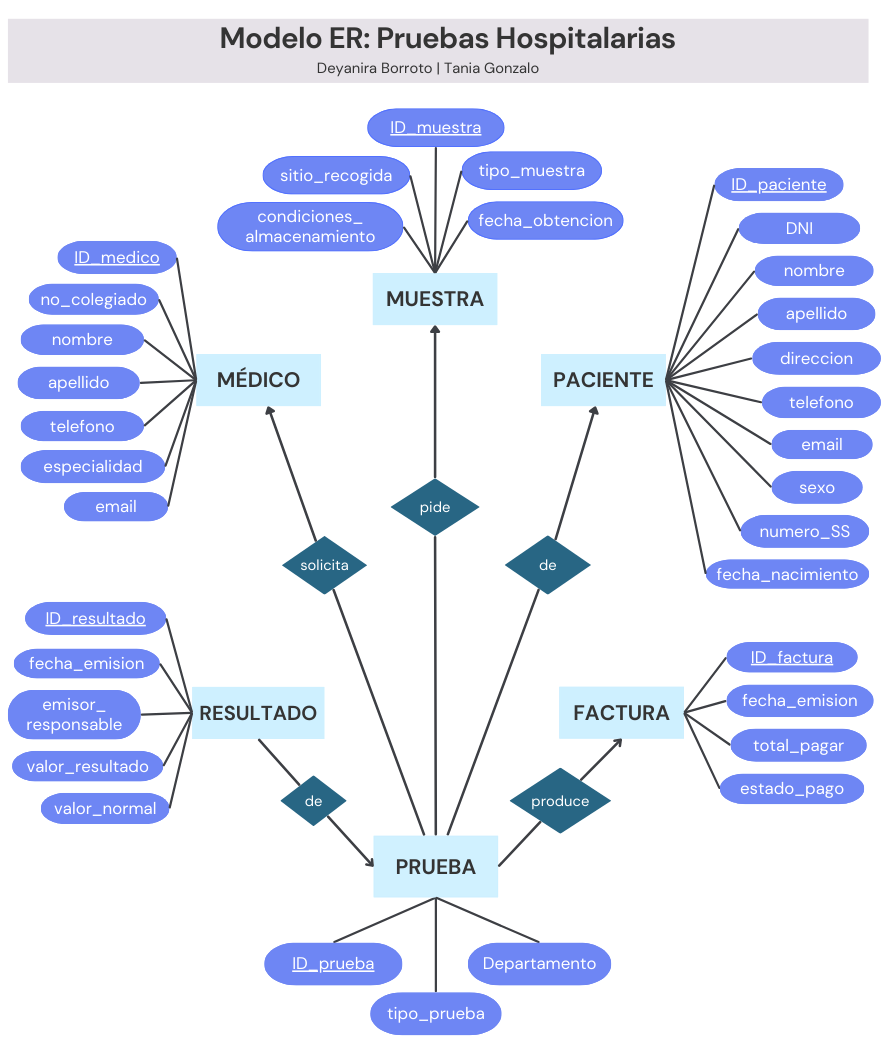
\includegraphics[width=150mm,scale=1.5]{Diagramas/diagramaER1.png}
    \caption{Diagrama ER de la base de datos de Pruebas Hospitalarias. \textit{Hecho en canva.com}}
    \label{fig:diagrama_er}
\end{figure}

\newpage
\section{Modelo relacional}
Una vez establecido el modelo conceptual (diagrama ER) para nuestra base de datos de Pruebas Hospitalarias, debemos transformarlo en un modelo lógico (tablas relacionales), el cual pueda ser manejado por los sistemas de gestión de bases de datos relacionales (SGBDR).

Esto es posible gracias a seguir unas reglas establecidas. Los pasos seguidos en nuestro caso se muestran en las seguientes secciones.

\subsection{Identificar claves primarias, entidades y relaciones N-N}
En la Tabla 2 se muestra un resumen de las entidades de nuestra base de datos junto con sus respectivas claves primarias. En nuestro caso, no tenemos relaciones N-N.

\begin{table}[h]
\center
\caption{Entidades y sus claves primeras correpondientes}
\label{tab:entrelac}
\begin{tabular}{@{}ll@{}}
\toprule
Entidad & Clave Primaria \\ \midrule
Paciente & ID\_paciente \\
Médico & ID\_medico \\
Prueba & ID\_prueba \\
Muestra & ID\_muestra \\
Resultado & ID\_resultado \\
Factura & ID\_factura \\ \bottomrule
\end{tabular}
\end{table}

Cada una de las entidades del diagrama ER se transformará en una tabla en el modelo relacional. Todas las relaciones en nuestro esquema son de tipo 1-N (uno a muchos). Este tipo de relaciones no se representan en forma de tabla como en el caso de las relaciones N-N, sino que se representan añadiendo una columna a la tabla correspondiente a la entidad del lado "muchos", la cual actuará como una clave foránea haciendo referencia a la clave primaria de la entidad del lado "uno".

\subsection{Modelo relacional}
Tras la identificaciones de las entidades con sus claves primeras y considernado las relaciones 1-N, obtener el modelo relacional de nuestra base de datos de Pruebas Hospitalarias es trivial. Se muestra a continuación:

\begin{itemize}
    \item \textbf{Paciente} (\underline{ID\_paciente}, nombre, apellido, DNI, dirección, telefono, email, fecha\_nacimiento, sexo, no\_seguridad\_social)
    \item \textbf{Médico} (\underline{ID\_medico}, nombre, apellido, no\_colegiado, telefono, email, especialidad)
    \item \textbf{Prueba} (\underline{ID\_prueba}, ID\_factura $\uparrow$, ID\_paciente $\uparrow$, ID\_muestra $\uparrow$, ID\_medico $\uparrow$, tipo\_prueba, departamento)
    \item \textbf{Muestra} (\underline{ID\_muestra}, fecha\_obtencion, sitio\_recogida, tipo\_muestra, condiciones\_almacenamiento)
    \item \textbf{Resultado} (\underline{ID\_resultado}, ID\_prueba $\uparrow$, fecha\_emisión, emisor\_responsable, valor\_normal, valor\_resultado)
    \item \textbf{Factura} (\underline{ID\_factura}, fecha\_emision, total\_pagar, estado\_pago)
\end{itemize}
    
Además, en la Figura 2 muestra el esquema tabular de nuestro modelo.

\newpage 

\begin{figure}[htbp]
    \centering
    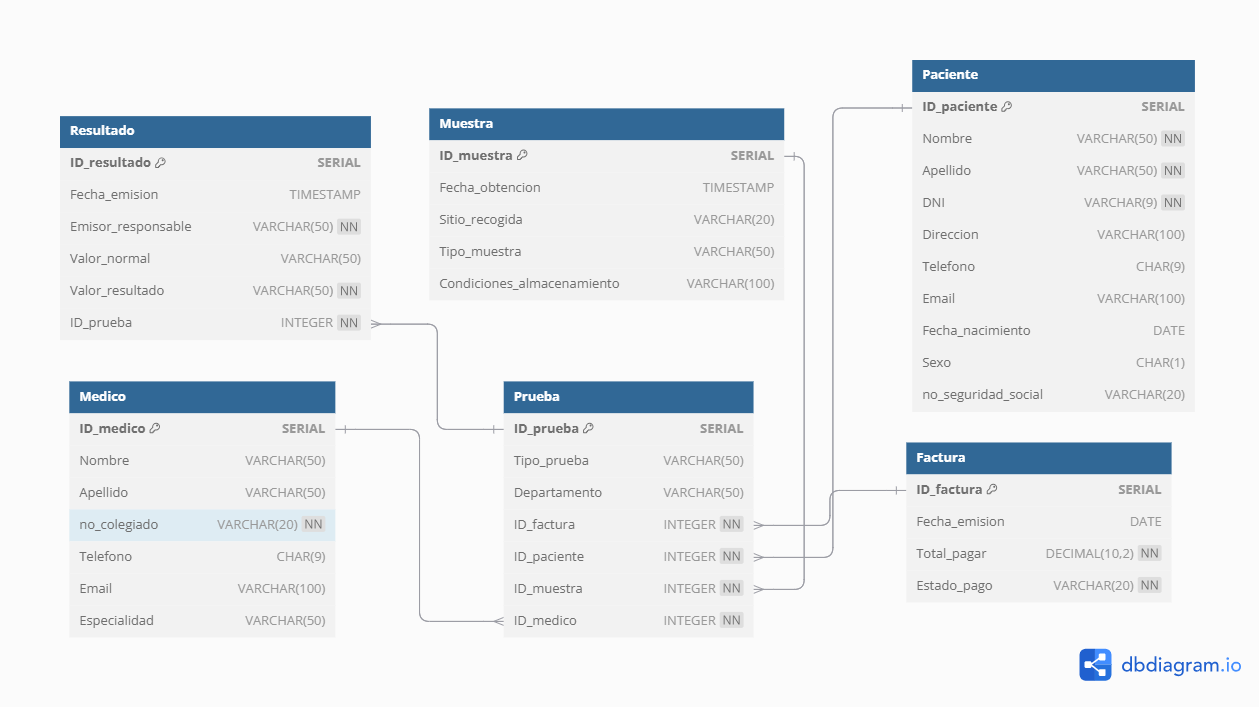
\includegraphics[width=0.9\textwidth]{Diagramas/Modelo_ER.png}
    \caption{Esquema tabular del diagrama ER de la base de datos de Pruebas Hospitalarias. \textit{Hecho en dbdiagram.io}}
    \label{fig:diagrama_er}
\end{figure}

\newpage
\section{Creación de tablas e inserción de datos}
Una vez obtenido el modelo de relaciones, la creación de tablas e inserción de datos se vuelve trivial gracias al lenguaje SQL. En nuestro caso, utilizamos PostgreSQL como sistema gestor de bases de datos (SGBD). El código SQL utilizado para la creación de las tablas se encuentra en el archivo \texttt{CREATE\_TABLES.sql}, mientras que los datos insertados están en el archivo \texttt{INSERTS\_TABLES.sql}.

A continuación, se describe la creación de cada una de las tablas y se muestra el resultado tras la inserción de los datos.


\subsection{Tabla Paciente}
La \textbf{tabla Paciente} almacena información sobre los pacientes, incluyendo su \texttt{ID\_paciente}, que es de tipo \texttt{SERIAL} y además actúa como clave primaria de la entidad. El resto de los atributos son: \texttt{Nombre} y \texttt{Apellido}, de tipo \texttt{VARCHAR(50)}, no pudiendo ser nulos; \texttt{DNI}, de tipo \texttt{VARCHAR(9)}, que no puede ser nulo y debe ser único; \texttt{Direccion} y \texttt{Email}, de tipo \texttt{VARCHAR(100)}; \texttt{Telefono}, de tipo \texttt{VARCHAR(9)}; \texttt{Fecha\_nacimiento}, de tipo \texttt{DATE}; \texttt{Sexo}, de tipo \texttt{CHAR(1)}; y \texttt{no\_seguridad\_social}, de tipo \texttt{VARCHAR(20)}. Además, mediante la restricción \texttt{CHECK}, se asegura que al menos uno de los campos de contacto (\texttt{Telefono} o \texttt{Email}) esté presente.

En esta tabla \textbf{Paciente} se realizaron 20 inserciones (archivo \texttt{INSERTS\_TABLES.sql}), obteniendo finalmente el resultado que se muestra en la Tabla 3.


\begin{table}[H]
\resizebox{\textwidth}{!}{%
\begin{tabular}{@{}|llllllllll|@{}}
\toprule
\textbf{\begin{tabular}[c]{@{}l@{}}id\_\\ paciente\end{tabular}} & \textbf{nombre} & \textbf{apellido} & \textbf{dni} & \textbf{direccion} & \textbf{telefono} & \textbf{email} & \textbf{\begin{tabular}[c]{@{}l@{}}fecha\_\\ nacimiento\end{tabular}} & \textbf{sexo} & \textbf{\begin{tabular}[c]{@{}l@{}}no\_seguridad\\ \_social\end{tabular}} \\ \hline
1 & Juan & Perez & 12113678A & Calle Alegria & 555123456 & NULL & 1960-01-01 & M & 123444789 \\ \hline
2 & Maria & Gamez & 87694521B & \begin{tabular}[c]{@{}l@{}}Avenida Plaza \\ Central\end{tabular} & NULL & maria@gmail.com & 1946-05-05 & F & NULL \\ \hline
3 & Marta & Maria & 87888881A & Calle Fuencarral & NULL & m.maria@gmail.com & 1956-05-05 & F & 155544789 \\ \hline
4 & Maria & Peres & 87421471W & Calle America & 656856789 & m.perez@educa.es & 1998-04-12 & F & 155544789 \\ \hline
5 & Lucia & Fernandez & 23731789C & Calle Real 145 & 555123789 & lucia@estudiante.uam.es & 1985-03-15 & F & 987653841 \\ \hline
6 & Miguel & Sanchez & 34426890D & Calle Mayor 101 & NULL & miguel\_san@gmail.com & 1950-07-20 & M & NULL \\ \hline
7 & Carlos & Ramirez & 12389678Z & Calle Sol 15 & 555987123 & NULL & 1982-06-15 & M & ABC123456 \\ \hline
8 & Ana & Santos & 87654321X & Avenida Luna 5 & NULL & ana.santos@gmail.com & 1990-02-20 & F & DEF987654 \\ \hline
9 & Pedro & Mendez & 23411189Y & Calle Estrella 9 & 555123654 & NULL & 1975-10-10 & M & GHI456789 \\ \hline
10 & Laura & Martinez & 98456632W & Plaza Mayor 2 & NULL & laura.martinez@gmail.com & 1988-08-25 & F & NULL \\ \hline
11 & Manuel & Vega & 34788890V & Calle Lluvia 33 & 555456987 & manuel.vega@hotmail.com & 1960-04-18 & M & JKL321987 \\ \hline
12 & Miguel & Vega & 54322278P & Calle Fuego 42 & 555789321 & NULL & 1992-12-12 & M & MNO654123 \\ \hline
13 & Ana & Saez & 11189611A & Calle Uno & 444489321 & NULL & 1981-03-05 & F & 111000111 \\ \hline
14 & Rebeca & Martin & 11777112A & Plaza Mayor & 111789321 & rebe\_martin@hotmail.com & 1981-01-01 & F & NULL \\ \hline
15 & Luis & Rodriguez & 87125521B & Calle Alegria & 554569321 & NULL & 1981-01-01 & M & 111258113 \\ \hline
16 & Ines & Gill & 11111114A & Calle Sonrisa & 555896321 & NULL & 1988-01-01 & F & 111251114 \\ \hline
17 & John & Dow & 23697189Y & Calle Sorolla & 111111321 & NULL & 1997-09-23 & M & 987653555 \\ \hline
18 & Laura & Perez & 23999189Y & Calle Pintor Rosales & 125896521 & lau\_perez@hotmail.com & 1981-12-15 & F & 987655555 \\ \hline
19 & Juan & Terez & 99911189Y & \begin{tabular}[c]{@{}l@{}}Calle Federico \\ Garcia Lorca\end{tabular} & 125659321 & juan\_terez@hotmail.com & 1985-01-20 & M & 987611111 \\ \hline
20 & Lorenzo & Garcia & 23331189Y & Calle Severo Ochoa & 789985321 & NULL & 1985-11-20 & F & NULL\\ \hline
\end{tabular}%
}
\caption{Contenido de la Tabla Paciente tras la inserción de datos.}
\label{tab:paciente}
\end{table}

 
\subsection{Tabla Médico}

La \textbf{tabla Medico} permite almacenar información sobre los médicos, incluyendo su \texttt{ID\_medico}, que es de tipo \texttt{SERIAL} y actúa como clave primaria de la entidad.El resto de atributos son: \texttt{Nombre} y \texttt{Apellido}, de tipo \texttt{VARCHAR(50)}; \texttt{no\_colegiado}, de tipo \texttt{VARCHAR(20)}, que no puede ser nulo y debe ser único; \texttt{Telefono}, de tipo \texttt{CHAR(9)}; \texttt{Email}, de tipo \texttt{VARCHAR(100)}; y \texttt{Especialidad}, de tipo \texttt{VARCHAR(50)}.

En esta tabla \textbf{Medico} se realizaron 20 inserciones (archivo \texttt{INSERTS\_TABLES.sql}), obteniendo finalmente el resultado que se muestra en la Tabla 4.

\begin{table}[H]
\resizebox{\textwidth}{!}{%
\begin{tabular}{@{}|lllllll|@{}}
\toprule
\textbf{id\_medico} & \textbf{nombre} & \textbf{apellido} & \textbf{no\_colegiado} & \textbf{telefono} & \textbf{email} & \textbf{especialidad} \\ \hline
1 & Dr. Carlos & Lopez & COL003 & 555654321 & carlos@centrosalud.com & Cardiologia \\ \hline
2 & Dra. Ana & Martinez & COL406 & 555987654 & ana@hotmail.com & Hematologia \\ \hline
3 & Dr. Pedro & Garcia & COL701 & 555321654 & pedro@gmail.com & Dermatologia \\ \hline
4 & Dra. Laura & Hernandez & COL012 & 555654987 & laura@gmail.com & Inmunologia \\ \hline
5 & Dr. Juan & Ramirez & COL004 & 555123456 & juan.ramirez@hospital.com & Cardiologia \\ \hline
6 & Dr. Alberto & Santos & COL543 & 555654321 & alberto.santos@hospital.com & Oncologia \\ \hline
7 & Dra. Juana & Lopez & COL987 & 955789123 & juana.lopez@hospital.com & Dermatologia \\ \hline
8 & Dra. Alejandra & Martinez & COL246 & 055321654 & alejandra.martinez@gmail.com & Neurologia \\ \hline
9 & Dra. Laura & Gonzalez & COL135 & 545987456 & laura.gonzalez@hotmail.com & Med.Interna \\ \hline
10 & Dr. Miguel & Ruiz & COL864 & 575654987 & miguel.ruiz@hospital.com & Oncologia \\ \hline
11 & Dr. Tio & Guay & COL111 & 218956111 & tioguay@gmail.com & Hematologia \\ \hline
12 & Dra. Lucy & Delight & COL112 & 221611481 & lucy@gmail.com & Cardiologia \\ \hline
13 & Dra. Pepi & Santana & COL113 & 231156111 & pepi@gmail.com & Med.General \\ \hline
14 & Dr. Keith & Sunny & COL114 & 241459611 & NULL & Hematologia \\ \hline
15 & Dr. John & Galea & COL115 & 251555611 & john@gmail.com & Med.General \\ \hline
16 & Dra. Jul & Step & COL116 & 261145661 & jul@gmail.com & Med.General \\ \hline
17 & Dra. Sand & Likelihood & COL117 & 271259811 & sand@gmail.com & Traumatologia \\ \hline
18 & Dr. Arbol & Lively & COL118 & 281658911 & arbol@gmail.com & Endocrinologia \\ \hline
19 & Dr. Trevor & Noah & COL119 & 291125411 & noah@gmail.com & Neumologia \\ \hline
20 & Dra. Sandra & Pepi & COL120 & 212125911 & sandra@gmail.com & Endocrinologia \\ \hline
\end{tabular}%
}
\caption{Contenido de la Tabla Médico tras la inserción de datos.}
\label{tab:medico}
\end{table}


\subsection{Tabla Prueba}

La \textbf{tabla Prueba} incluye información sobre las pruebas realizadas y permite la relación con los pacientes, médicos, muestras y facturas correspondientes. Como atributos tenemos su \texttt{ID\_prueba}, que es de tipo \texttt{SERIAL} y actúa como clave primaria de la entidad. Los demás atributos son: \texttt{Tipo\_prueba}, de tipo \texttt{VARCHAR(50)}; \texttt{Departamento}, de tipo \texttt{VARCHAR(50)}; \texttt{ID\_factura}, de tipo \texttt{INTEGER}, que referencia a \texttt{Factura(ID\_factura)} y no puede ser nulo; \texttt{ID\_paciente}, de tipo \texttt{INTEGER}, que referencia a \texttt{Paciente(ID\_paciente)} y no puede ser nulo; \texttt{ID\_muestra}, de tipo \texttt{INTEGER}, que referencia a \texttt{Muestra(ID\_muestra)} y no puede ser nulo; y \texttt{ID\_medico}, de tipo \texttt{INTEGER}, que referencia a \texttt{Medico(ID\_medico)} y no puede ser nulo.

En esta tabla \textbf{Prueba} se realizaron 28 inserciones (archivo \texttt{INSERTS\_TABLES.sql}), obteniendo finalmente el resultado que se muestra en la Tabla 5.

\begin{table}[H]
\resizebox{\textwidth}{!}{%
\begin{tabular}{@{}|lllllll|@{}}
\toprule
\textbf{id\_prueba} & \textbf{tipo\_prueba} & \textbf{departamento} & \textbf{id\_factura} & \textbf{id\_paciente} & \textbf{id\_muestra} & \textbf{id\_medico} \\ \hline
1 & Electrocardiograma & Cardiologia & 1 & 1 & 1 & 1 \\ \hline
2 & Coagulacion & Bioquimica & 2 & 2 & 2 & 2 \\ \hline
3 & Biopsia de piel & Patologia & 3 & 3 & 3 & 3 \\ \hline
4 & Serologia & Bioquimica & 4 & 4 & 4 & 4 \\ \hline
5 & Analitica & Hematologia & 5 & 5 & 5 & 5 \\ \hline
6 & Holter & Cardiologia & 6 & 6 & 6 & 5 \\ \hline
7 & Biopsia & Patologia & 7 & 7 & 7 & 6 \\ \hline
8 & Electrocardiograma & Cardiologia & 8 & 8 & 8 & 5 \\ \hline
9 & Prueba de esfuerzo & Deporte & 9 & 9 & 9 & 9 \\ \hline
10 & Biopsia & Patologia & 10 & 10 & 10 & 10 \\ \hline
11 & Analitica & Hematologia & 11 & 11 & 11 & 11 \\ \hline
12 & Holter & Cardiologia & 11 & 11 & 23 & 12 \\ \hline
13 & Analitica & Hematologia & 12 & 12 & 12 & 12 \\ \hline
14 & Biopsia & Patologia & 13 & 13 & 13 & 13 \\ \hline
15 & Analitica & Hematologia & 1 & 1 & 1 & 13 \\ \hline
16 & Hematologia & Hematologia & 14 & 14 & 14 & 14 \\ \hline
17 & Coagulacion & Bioquimica & 1 & 1 & 1 & 14 \\ \hline
18 & Serologia & Bioquimica & 2 & 2 & 2 & 14 \\ \hline
19 & Analitica & Hematologia & 15 & 15 & 15 & 15 \\ \hline
20 & Microbiología & Microbiología & 15 & 15 & 15 & 15 \\ \hline
21 & Biopsia & Patologia & 16 & 16 & 16 & 16 \\ \hline
22 & Rayos X & Radiologia & 17 & 17 & 17 & 17 \\ \hline
23 & Hormonas & Endocrinologia & 18 & 18 & 18 & 18 \\ \hline
24 & Espirometria & Neumologia & 19 & 19 & 19 & 19 \\ \hline
25 & Ecografia de cuello & Radiologia & 20 & 20 & 24 & 20 \\ \hline
26 & Analitica & Hematologia & 20 & 20 & 20 & 1 \\ \hline
27 & Biopsia de piel & Patologia & 1 & 1 & 21 & 7 \\ \hline
28 & Escaner & Radiologia & 7 & 7 & 22 & 8 \\ \hline
\end{tabular}%
}
\caption{Contenido de la Tabla Prueba tras la inserción de datos.}
\label{tab:prueba}
\end{table}


\subsection{Tabla Muestra}

La \textbf{tabla Muestra} permite almacenar información sobre las muestras recogidas, incluyendo su \texttt{ID\_muestra}, que es de tipo \texttt{SERIAL} y actúa como clave primaria de la entidad. El resto de atributos son: \texttt{Fecha\_obtencion}, de tipo \texttt{TIMESTAMP}; \texttt{Sitio\_recogida}, de tipo \texttt{VARCHAR(20)}; \texttt{Tipo\_muestra}, de tipo \texttt{VARCHAR(50)}; y \texttt{Condiciones\_almacenamiento}, de tipo \texttt{VARCHAR(100)}, pudiendo todos estos atributos (menos la clave primaria) ser nulos.

En esta tabla \textbf{Muestra} se realizaron 24 inserciones (archivo \texttt{INSERTS\_TABLES.sql}), obteniendo finalmente el resultado que se muestra en la Tabla 6.

\begin{table}[H]
\resizebox{\textwidth}{!}{%
\begin{tabular}{@{}|lllll|@{}}
\toprule
\textbf{id\_muestra} & \textbf{fecha\_obtencion} & \textbf{sitio\_recogida} & \textbf{tipo\_muestra} & \textbf{condiciones\_almacenamiento}  \\ \hline
1 & 2024-06-01 08:00:00 & Extracciones & Sangre & Refrigerado \\ \hline
2 & 2024-06-01 08:00:00 & Extracciones & Sangre & Refrigerado \\ \hline
3 & 2024-06-02 08:00:00 & Quirofano1 & Tejido & Congelado \\ \hline
4 & 2024-06-04 08:00:00 & Extracciones & Sangre & Congelado \\ \hline
5 & 2024-06-05 08:00:00 & Laboratorio Central & Sangre & Temperatura ambiente \\ \hline
6 & NULL & NULL & NULL & NULL \\ \hline
7 & 2024-06-05 08:00:00 & Quirofano1 & Tejido & Congelado \\ \hline
8 & NULL & NULL & NULL & NULL \\ \hline
9 & NULL & NULL & NULL & NULL \\ \hline
10 & 2024-06-06 08:00:00 & Quirofano3 & Tejido & Congelado \\ \hline
11 & 2024-06-07 08:30:00 & Extracciones & Sangre & Temperatura ambiente \\ \hline
12 & 2024-06-08 08:20:00 & Extracciones & Sangre & Temperatura ambiente \\ \hline
13 & 2024-06-10 08:16:00 & Quirofano4 & Tejido & Congelado \\ \hline
14 & 2024-06-11 08:16:00 & Extracciones & Sangre & Temperatura ambiente \\ \hline
15 & 2024-06-21 07:00:00 & Extracciones & Sangre & Temperatura ambiente \\ \hline
16 & 2024-06-22 09:00:00 & Quirofano2 & Tejido & Congelado \\ \hline
17 & NULL & NULL & NULL & NULL \\ \hline
18 & 2024-06-12 10:00:00 & Extracciones & Sangre & Refrigerado \\ \hline
19 & NULL & NULL & NULL & NULL \\ \hline
20 & 2024-06-13 18:00:00 & Extracciones & Sangre & Temperatura ambiente \\ \hline
21 & 2024-06-14 20:00:00 & Quirofano1 & Tejido & Congelado \\ \hline
22 & NULL & NULL & NULL & NULL \\ \hline
23 & NULL & NULL & NULL & NULL \\ \hline
24 & NULL & NULL & NULL & NULL  \\ \hline
\end{tabular}%
}
\caption{Contenido de la Tabla Muestra tras la inserción de datos.}
\label{tab:muestra}
\end{table}


\subsection{Tabla Factura}

La \textbf{tabla Factura} permite almacenar información sobre las facturas emitidas. Incluye su \texttt{ID\_factura}, que es de tipo \texttt{SERIAL} y actúa como clave primaria de la entidad. El resto de atributos son: \texttt{Fecha\_emision}, de tipo \texttt{DATE}; \texttt{Total\_pagar}, de tipo \texttt{DECIMAL(10, 2)}, que no puede ser nulo; y \texttt{Estado\_pago}, de tipo \texttt{VARCHAR(20)}, que tampoco puede ser nulo.

En esta tabla \textbf{Factura} se realizaron 20 inserciones (archivo \texttt{INSERTS\_TABLES.sql}), obteniendo finalmente el resultado que se muestra en la Tabla 7.

\begin{table}[H]
\centering
\begin{tabular}{@{}|llll|@{}}
\toprule
\textbf{id\_factura} & \textbf{fecha\_emision} & \textbf{total\_pagar} & \textbf{estado\_pago} \\
\hline
1 & 2024-09-20 & 150.75 & Pagado \\ \hline
2 & 2024-09-21 & 200.00 & Pendiente \\ \hline
3 & 2024-09-24 & 75.50 & Pagado \\ \hline
4 & 2024-09-25 & 120.00 & Pendiente \\ \hline
5 & 2024-09-15 & 50.75 & Pagado \\ \hline
6 & 2024-09-20 & 100.00 & Pendiente \\ \hline
7 & 2024-09-05 & 175.50 & Pagado \\ \hline
8 & 2024-09-12 & 220.00 & Pendiente \\ \hline
9 & 2024-10-10 & 300.25 & Pagado \\ \hline
10 & 2024-10-01 & 150.00 & Pendiente \\ \hline
11 & 2024-10-04 & 400.00 & Pendiente \\ \hline
12 & 2024-10-16 & 300.00 & Pagado \\ \hline
13 & 2024-10-18 & 200.00 & Pagado \\ \hline
14 & 2024-10-20 & 410.99 & Pagado \\ \hline
15 & 2024-10-01 & 340.99 & Pendiente \\ \hline
16 & 2024-10-01 & 400.00 & Pendiente \\ \hline
17 & 2024-10-01 & 110.00 & Pendiente \\ \hline
18 & 2024-10-01 & 400.00 & Pagado \\ \hline
19 & 2024-10-01 & 210.00 & Pendiente \\ \hline
20 & 2024-10-01 & 520.00 & Pagado \\ \hline
\end{tabular}
\caption{Contenido de la Tabla Factura tras la inserción de datos.}
\label{tab:factura}
\end{table}


\subsection{Tabla Resultado}

La \textbf{tabla Resultado} almacena los resultados de las pruebas. Incluye su \texttt{ID\_resultado}, que es de tipo \texttt{SERIAL} y actúa como clave primaria de la entidad. Los demás atributos son: \texttt{Fecha\_emision}, de tipo \texttt{TIMESTAMP}; \texttt{Emisor\_responsable}, de tipo \texttt{VARCHAR(50)}, que no puede ser nulo; \texttt{Valor\_normal}, de tipo \texttt{VARCHAR(50)}; \texttt{Valor\_resultado}, de tipo \texttt{VARCHAR(50)}, que no puede ser nulo; y \texttt{ID\_prueba}, de tipo \texttt{INTEGER}, que referencia a \texttt{Prueba(ID\_prueba)} y no puede ser nulo.

En esta tabla \textbf{Resultado} se realizaron 35 inserciones (archivo \texttt{INSERTS\_TABLES.sql}), obteniendo finalmente el resultado que se muestra en la Tabla 8.

\begin{table}[H]
\resizebox{\textwidth}{!}{%
\begin{tabular}{@{}|llllll|@{}}
\toprule
\textbf{\begin{tabular}[c]{@{}l@{}}id\_\\ resultado\end{tabular}} & \textbf{fecha\_emision} & \textbf{emisor\_responsable} & \textbf{valor\_normal} & \textbf{valor\_resultado} & \textbf{\begin{tabular}[c]{@{}l@{}}id\_\\ prueba\end{tabular}} \\ \hline
1 & 2024-07-01 10:00:00 & Dra. Raquel Aguado & Rango Normal & Rango Normal & 1 \\ \hline
2 & 2024-07-02 10:00:00 & Dr. José Izquierdo & Negativo & Negativo & 2 \\ \hline
3 & 2024-07-20 10:00:00 & Dr. José Izquierdo & Negativo & Positivo & 2 \\ \hline
4 & 2024-07-21 10:00:00 & Dra. Eva Iglesias & Negativo & Negativo & 3 \\ \hline
5 & 2024-07-10 10:00:00 & Dra. Ana Segundo & Positivo & Negativo & 4 \\ \hline
6 & 2024-08-26 09:00:00 & Dra. Ana Segundo & Positivo & Negativo & 4 \\ \hline
7 & 2024-07-23 10:00:00 & Dra. Nerea Sanchez & Rango Normal & Rango Normal & 5 \\ \hline
8 & 2024-07-16 10:00:00 & Dr. Carlos Ramirez & Rango Normal & Anomalia & 6 \\ \hline
9 & 2024-07-15 10:00:00 & Dra. Ana Santos & Normal & Malignidad & 7 \\ \hline
10 & 2024-07-13 10:00:00 & Dr. Pedro Lopez & Rango Normal & Onda T alterada & 8 \\ \hline
11 & 2024-07-12 10:00:00 & Dra. Laura Martinez & Normal & Normal & 9 \\ \hline
12 & 2024-07-11 10:00:00 & Dr. Manuel Gonzalez & Normal & Benigno & 10 \\ \hline
13 & 2024-08-18 10:00:00 & Dra. Elena Ruiz & Rango Normal & Colesterol alto & 11 \\ \hline
14 & 2024-07-20 10:00:00 & Dra. Elena Ruiz & Rango Normal & Trigliceridos altos & 11 \\ \hline
15 & 2024-07-21 10:00:00 & Dra. Elena Ruiz & Rango Normal & Rango Normal & 11 \\ \hline
16 & 2024-07-26 10:00:00 & Dr. Carlos Lopez & Rango Normal & Rango Normal & 12 \\ \hline
17 & 2024-07-30 10:00:00 & Dra. Ana Martinez & Rango Normal & Rango Normal & 13 \\ \hline
18 & 2024-07-30 10:00:00 & Dra. Ana Lopez & Normal & Malignidad & 14 \\ \hline
19 & 2024-07-31 10:00:00 & Dra. Juana Garcia & Rango Normal & \begin{tabular}[c]{@{}l@{}}Transaminasas\\ altas\end{tabular} & 15 \\ \hline
20 & 2024-07-16 10:00:00 & Dra. Juana Garcia & Rango Normal & Glucosa baja & 15 \\ \hline
21 & 2024-07-05 10:00:00 & Dr. Pedro Arroba & Negativo & Negativo & 16 \\ \hline
22 & 2024-07-06 10:00:00 & Dr. Juan Gonzalez & 0.9 & 0.9 & 17 \\ \hline
23 & 2024-07-20 10:00:00 & Dr. Federico Roldan & Negativo & Positivo & 18 \\ \hline
24 & 2024-07-08 10:00:00 & Dr. Miguel Galan & Rango Normal & Rango Normal & 19 \\ \hline
25 & 2024-07-07 10:00:00 & Dr. Miguel Galan & Rango Normal & Celiaquia & 19 \\ \hline
26 & 2024-07-16 10:00:00 & Dr. Jose Pedro Sanz & Positivo & Negativo & 20 \\ \hline
27 & 2024-07-16 10:00:00 & Dr. Jose Pedro Sanz & Positivo & Positivo & 20 \\ \hline
28 & 2024-07-18 10:00:00 & \begin{tabular}[c]{@{}l@{}}Dra. Maria del Mar\\ Sanchez\end{tabular} & Normal & Benigno & 21 \\ \hline
29 & 2024-07-10 10:00:00 & Dra. Estrella Aguado & Normal & Fractura & 22 \\ \hline
30 & 2024-07-22 10:00:00 & Dra. Eva Perez & Normal & TSH alta & 23 \\ \hline
31 & 2024-07-28 09:32:00 & Dra. Sara Gala & Normal & Normal & 24 \\ \hline
32 & 2024-07-25 10:32:00 & Dr. Manuel Romero & Normal & Nodulos & 25 \\ \hline
33 & 2024-07-23 11:26:00 & Dr. Oscar Lafuente & Normal & Normal & 26 \\ \hline
34 & 2024-07-29 11:26:00 & Dr. Juan Perez & Normal & Benigno & 27 \\ \hline
35 & 2024-07-28 11:26:00 & Dra. Lucia Pau & Normal & Normal & 28 \\ \hline
\end{tabular}%
}
\caption{Contenido de la Tabla Resultado tras la inserción de datos.}
\label{tab:resultado}
\end{table}

\newpage
\section{Consultas de ejemplo y resultados}
En esta sección se presentan algunas consultas avanzadas que se pueden realizar en nuestra base de datos de pruebas hospitalarias. Estas consultas permiten extraer información útil y compleja, aprovechando las relaciones entre las tablas, poniendo en evidencia la relevancia de las bases de datos en este campo. 

El código SQL de cada una de las consultas que se describen a continuación se encuentra en el archivo \texttt{QUERIES.sql}.



\subsection{Recuperar pacientes con más de una muestra mayores de 50 años.}

\textbf{Consulta SQL}
\begin{lstlisting}[language=SQL]
SELECT Paciente.Nombre AS nombre_paciente, Paciente.Apellido AS apellido_paciente, EXTRACT(YEAR FROM AGE(Paciente.Fecha_nacimiento)) AS edad, COUNT(DISTINCT Muestra.ID_muestra) AS Numero_Muestras
FROM Paciente
JOIN Prueba ON Paciente.ID_paciente = Prueba.ID_paciente
JOIN Muestra ON Prueba.ID_muestra = Muestra.ID_muestra
WHERE EXTRACT(YEAR FROM AGE(Paciente.Fecha_nacimiento)) > 50
GROUP BY Paciente.Nombre, Paciente.Apellido, Paciente.Fecha_nacimiento
HAVING COUNT(DISTINCT Muestra.ID_muestra) > 1
ORDER BY Numero_Muestras DESC;
\end{lstlisting}

\textbf{Explicación de la consulta SQL}

Esta consulta recupera el número de muestras distintas asociadas a cada paciente mayor de 50 años. Para ello, se realiza la unión de las tablas \textbf{Paciente}, \textbf{Prueba} y \textbf{Muestra} mediante las claves \texttt{ID\_paciente} y \texttt{ID\_muestra}. Posteriormente, se filtran los pacientes mayores de 50 años utilizando la cláusula \texttt{WHERE}, que aplica la función \texttt{EXTRACT(YEAR FROM AGE(...))} para calcular la edad del paciente a partir de su fecha de nacimiento. Los resultados se agrupan por paciente mediante la cláusula \texttt{GROUP BY}, utilizando como identificadores únicos su nombre, apellido y fecha de nacimiento. A continuación, se filtran los grupos para incluir únicamente aquellos pacientes con más de una muestra registrada, utilizando la cláusula \texttt{HAVING}. Finalmente, los resultados se ordenan de manera descendente según la cantidad de muestras distintas mediante la cláusula \texttt{ORDER BY}, priorizando así los pacientes con más material disponible.

\textbf{Resultado de la consulta}

La salida de la consulta muestra los pacientes mayores de 50 años que tienen más de una muestra registrada en la base de datos como vemos en la Tabla 9.

\begin{table}[h!]
\centering
\begin{tabular}{|c|c|c|c|}
\hline
\textbf{nombre\_paciente} & \textbf{apellido\_paciente} & \textbf{edad} & \textbf{numero\_muestras} \\
\hline
Juan & Perez & 64 & 2 \\
\hline
Manuel & Vega & 64 & 2 \\
\hline
\end{tabular}
\caption{Pacientes con más de una muestra mayores de 50 años}
\label{tab:pacientes_muestras}
\end{table}

\textbf{Interpretación}

La salida de la consulta muestra el nombre y apellido del paciente, su edad y el número de muestras distintas que tienen. En nuestro caso, existen dos pacientes en nuestra base de datos: \textbf{Juan Pérez} y \textbf{Manuel Vega}, ambos de 64 años, cada uno con 2 muestras distintas recogidas. 

Esto indica que en el laboratorio tenemos material adicional disponible para estos pacientes, lo cual podría ser útil en caso de necesitar realizar pruebas complementarias.


\subsection{Facturas pendientes de pago con un total a pagar superior a 300}

\textbf{Consulta SQL}
\begin{lstlisting}[language=SQL]
SELECT 
    Paciente.Nombre AS nombre_paciente, 
    Paciente.Apellido AS apellido_paciente, 
    Factura.Total_pagar AS Pendiente_pago
FROM Paciente
JOIN Prueba ON Paciente.ID_paciente = Prueba.ID_paciente
JOIN Factura ON Prueba.ID_factura = Factura.ID_factura
WHERE Factura.Estado_pago = 'Pendiente' AND Factura.Total_pagar > 300
GROUP BY Paciente.Nombre, Paciente.Apellido, Factura.Total_pagar
ORDER BY Pendiente_pago DESC;
\end{lstlisting}

\textbf{Explicación de la consulta SQL}

Esta consulta recupera el nombre y apellido de los pacientes, junto con el total pendiente de pago de las facturas, ordenados de manera descendente según el total a pagar pendiente. Para ello, se realiza la unión de las tablas \textbf{Paciente}, \textbf{Prueba} y \textbf{Factura} mediante las claves \texttt{ID\_paciente} e \texttt{ID\_factura}. La cláusula \texttt{WHERE} filtra los resultados para incluir solo los pacientes que deben pagar más de 300 (\texttt{Total\_pagar > 300}) y las facturas cuyo estado de pago es \texttt{'Pendiente'}. Los resultados se agrupan por paciente y total pendiente de pago utilizando la cláusula \texttt{GROUP BY}. Finalmente se ordenan según el total a pagar pendiente mediante la cláusula \texttt{ORDER BY}.

\textbf{Resultado de la consulta}

Como podemos observar en la Tabla 10, la consulta devuelve los nombres y apellidos de los pacientes que tienen facturas pendientes de pago con un total a pagar superior a 300.00.

\begin{table}[h!]
\centering
\begin{tabular}{|c|c|c|}
\hline
\textbf{nombre\_paciente} & \textbf{apellido\_paciente} & \textbf{pendiente\_pago} \\
\hline
Ines & Gill & 400.00 \\
\hline
Manuel & Vega & 400.00 \\
\hline
Luis & Rodriguez & 340.99 \\
\hline
\end{tabular}
\caption{Pacientes con facturas pendientes de pago mayores a 300.00.}
\label{tab:facturas_pendientes}
\end{table}


\textbf{Interpretación}
Los resultados muestran a los pacientes con su respectiva cantidad de pagar pendiente. En nuestro caso, vemos que solo tenemos tres pacientes, de los cuales \textbf{Ines Gill} y \textbf{Manuel Vega} tiene pendiente pagar un total de 400, mientras que \textbf{Luis Rodriguez} tiene utiene pendiente pagar un total de 340.99.

Esta información facilita la gestión de cuentas por cobrar con valores elevados (superiores a 300) que todavía no han sido pagadas. 

\subsection{Obtener el historial de pruebas y resultados de un paciente específico.}

\textbf{Consulta SQL}
\begin{lstlisting}[language=SQL]
SELECT 
    p.Nombre, p.Apellido, pr.Tipo_prueba, r.Fecha_emision, r.Valor_resultado
FROM Paciente p
JOIN Prueba pr ON p.ID_paciente = pr.ID_paciente
JOIN Resultado r ON pr.ID_prueba = r.ID_prueba
WHERE p.DNI = '12113678A'
ORDER BY r.Fecha_emision DESC;
\end{lstlisting}

\newpage
\textbf{Explicación de la consulta SQL}

La consulta permite recuperar el historial de pruebas y resultados de un paciente específico identificado por su DNI. Para ello, se realiza la unión de las tablas \textbf{Paciente}, \textbf{Prueba} y \textbf{Resultado} mediante las claves \texttt{ID\_paciente} y \texttt{ID\_prueba}. Se utiliza la cláusula \texttt{JOIN} para combinar las tablas y la cláusula \texttt{WHERE} para filtrar los resultados basados en el DNI del paciente. La cláusula \texttt{SELECT} permite elegir las columnas relevantes, como el nombre y apellido del paciente, el tipo de prueba, la fecha de emisión y el valor del resultado. Además, se ordena por fecha de emision del resultado de la prueba mediante \texttt{ORDER BY} de más reciente a más antigua.

\textbf{Resultado de la consulta}

La salida de la consulta muestra el historial de pruebas y resultados del paciente Juan Perez, con el DNI \texttt{'12113678A'}. Los resultados incluyen el tipo de prueba, la fecha de emisión y el valor del resultado de cada prueba realizada como podemos observar en la Tabla 11.

\begin{table}[h!]
\centering
\begin{tabular}{|c|c|c|c|c|}
\hline
\textbf{nombre} & \textbf{apellido} & \textbf{tipo\_prueba} & \textbf{fecha\_emision} & \textbf{valor\_resultado} \\
\hline
Juan & Perez & Analítica & 2024-07-31 10:00:00 & Transaminasas altas \\
Juan & Perez & Biopsia de piel & 2024-07-29 11:26:00 & Benigno \\
Juan & Perez & Analítica & 2024-07-16 10:00:00 & Glucosa baja \\
Juan & Perez & Coagulación & 2024-07-06 10:00:00 & 0.9 \\
Juan & Perez & Electrocardiograma & 2024-07-01 10:00:00 & Rango Normal \\
\hline
\end{tabular}
\caption{Historial de pruebas y resultados del paciente con DNI '12113678A'}
\label{tab:historial_prueba}
\end{table}

\textbf{Interpretación}

En este caso podemos observar el historial de pruebas y resultados del paciente \textbf{Juan Perez}, con DNI \texttt{'12113678A'}. La tabla muestra las pruebas realizadas a este paciente como por ejemplo un electrocardiograma con resultado de \texttt{Rango Normal}, y una analítica con resultados de \texttt{Transaminasas altas}, entre otros. 

Esta información podría ser crucial para el seguimiento de la salud del paciente y para los médicos al revisar los resultados anteriores y tomar decisiones informadas.

\subsection{Importe de las pruebas solicitadas por cada uno de los médicos en la segunda quincena de septiembre de 2024 ordenado por dia.}

\textbf{Consulta SQL}
\begin{lstlisting}[language=SQL]
SELECT m.Nombre AS nombre_medico, 
       TO_CHAR(f.Fecha_emision, 'DD') AS Dia, 
       f.Total_pagar AS importe_por_pruebas_solicitadas
FROM Factura f
JOIN Prueba p ON p.id_factura = f.id_factura
JOIN Medico m ON p.id_medico = m.ID_medico 
WHERE f.Fecha_emision BETWEEN '2024-09-15' AND '2024-09-30'
GROUP BY m.Nombre, TO_CHAR(f.Fecha_emision, 'DD'), f.Total_pagar
ORDER BY Dia ASC;
\end{lstlisting}

\textbf{Explicación de la consulta SQL}

La consulta obtiene el nombre de los médicos, el día del mes de la fecha de emisión y el importe por las pruebas solicitadas en un período específico. Se realiza la unión de las tablas \textbf{Factura}, \textbf{Prueba} y \textbf{Medico} mediante las claves \texttt{id\_factura} y \texttt{id\_medico}. La cláusula \texttt{JOIN} se utiliza para combinar las tablas y \texttt{SELECT} para elegir las columnas relevantes, como el nombre del médico, el día de la emisión y el importe total de la factura. La cláusula \texttt{WHERE} filtra los resultados para incluir solo aquellas facturas emitidas entre el 15 y el 30 de septiembre de 2024. Los resultados se agrupan por el nombre del médico, el día de la emisión y el importe, utilizando la cláusula \texttt{GROUP BY}, y se ordenan por día de manera ascendente con la cláusula \texttt{ORDER BY}.

\textbf{Resultado de la consulta}

La salida de la consulta (Tabla 12) muestra los nombres de los médicos, el día de la fecha de emisión y el importe por las pruebas solicitadas dentro del período comprendido entre el 15 y el 30 de septiembre de 2024. 

\begin{table}[h!]
\centering
\begin{tabular}{|c|c|c|}
\hline
\textbf{nombre\_medico} & \textbf{dia} & \textbf{importe\_por\_pruebas\_solicitadas} \\
\hline
Dr. Juan & 15 & 50.75 \\ \hline
Dr. Carlos & 20 & 150.75 \\ \hline
Dr. Juan & 20 & 100.00 \\ \hline
Dr. Keith & 20 & 200.00 \\ \hline
Dra. Juana & 20 & 150.75 \\ \hline
Dra. Pepi & 20 & 150.75 \\ \hline
Dr. Keith & 21 & 200.00 \\ \hline
Dra. Ana & 21 & 200.00 \\ \hline
Dr. Pedro & 24 & 75.50 \\ \hline
Dra. Laura & 30 & 120.00 \\ \hline
\end{tabular}
\caption{Importe diario de pruebas solicitadas por médicos en la segunda quincena de septiembre de 2024}
\label{tab:historial_prueba}
\end{table}

\textbf{Interpretación}

En este caso, podemos observar el dia 15 de septiembre se emitió una factura asociada al \texttt{Dr. Juan} asociada a un importe total a pagar de 50.75, mientras que el 30 de septiembre se emitió una factura asociada a la \texttt{Dra. Laura} asociada a un importe total a pagar de 120.00. 

Esta consulta permite obtener el importe por pruebas solicitadas asociadas a cada uno de los médicos por dia, pudiendo esto ser de utilidad para la gestión de gastos del hospital. 


\subsection{El paciente con más pruebas realizadas a partir de una única muestra que debe mantenerse o bien refrigeradas o bien congeladas.}

\textbf{Consulta SQL}
\begin{lstlisting}[language=SQL]
SELECT p.nombre AS nombre_paciente, 
       m.Tipo_muestra, 
       m.Condiciones_almacenamiento, 
       COUNT(pr.ID_prueba) AS Numero_Pruebas
FROM Muestra m
JOIN Prueba pr ON m.ID_muestra = pr.ID_muestra
JOIN Paciente p ON p.ID_paciente = pr.ID_paciente
WHERE LOWER(m.Condiciones_almacenamiento) LIKE '%refrigerado%' 
   OR LOWER(m.Condiciones_almacenamiento) LIKE '%congelado%'
GROUP BY m.ID_muestra, m.Tipo_muestra, m.Condiciones_almacenamiento, p.nombre
HAVING COUNT(pr.ID_prueba) > 1
ORDER BY Numero_Pruebas DESC
LIMIT 1;
\end{lstlisting}

\textbf{Explicación de la consulta SQL}

Esta consulta tiene como objetivo encontrar el paciente con el mayor número de pruebas realizadas a partir de una única muestra que debe mantenerse o bien refrigerada o bien congelada. Para ello, seleccionamos varias columnas: el nombre del paciente, el tipo de muestra, las condiciones de almacenamiento y el número de pruebas realizadas. Posteirormente, se usa \texttt{JOIN} para combinar las tablas \textbf{Muestra}, \textbf{Prueba} y \textbf{Paciente}. La cláusula \texttt{WHERE} permite filtrar las muestras que deben mantenerse o bien refrigeradas o bien congeladas, y se emplea la función \texttt{COUNT} para contar las pruebas asociadas a cada muestra. Luego, los resultados se agrupan por muestra, tipo de muestra, condiciones de almacenamiento y nombre del paciente mediante la cláusula \texttt{GROUP BY}, y se filtran para mostrar solo aquellos pacientes con más de una prueba mediante la cláusula \texttt{HAVING}. Finalmente, se ordenan los resultados de manera descendente por el número de pruebas realizadas y se limita la salida a un solo registro utilizando \texttt{LIMIT 1}.

\textbf{Resultado de la consulta}

Como vemos en la Tabla 13, la salida de la consulta muestra el nombre del paciente, el tipo de muestra, las condiciones de almacenamiento y el número de pruebas realizadas para la muestra que debe mantenerse refrigerada o congelada. 

\begin{table}[h!]
\centering
\begin{tabular}{|c|c|c|c|}
\hline
\textbf{nombre\_paciente} & \textbf{tipo\_muestra} & \textbf{condiciones\_almacenamiento} & \textbf{numero\_pruebas} \\
\hline
Juan & Sangre & Refrigerado & 3 \\
\hline
\end{tabular}
\caption{Pacientes con mayor cantidad de pruebas realizadas a partir de una única muestra que requiere refrigeración o congelación.}
\label{tab:historial_prueba}
\end{table}

\textbf{Interpretación}

En este caso, el paciente con más pruebas realizadas a aprtir de una muestra es \texttt{Juan}, quien tiene una muestra de sangre que debe mantenerse refrigerada. El total de pruebas realizadas con esa muestra es de 3. 

Esta información es importante para conocer la carga de pruebas asociada a un tipo específico de muestra, lo que puede ser relevante a nivel médico y gestión hospitalaria.


\subsection{Obtener el primer médico ordenado por apellido junto con su número de pruebas del departamento con más pruebas solicitadas.}

\textbf{Consulta SQL}
\begin{lstlisting}[language=SQL]
SELECT m.Nombre AS nombre_medico, 
       m.Apellido AS apellido_medico, 
       COUNT(p.ID_prueba) AS Numero_Pruebas
FROM Medico m
JOIN Prueba p ON m.ID_medico = p.ID_medico
WHERE p.Departamento = (
        SELECT p1.Departamento
        FROM Prueba p1
        GROUP BY p1.Departamento
        ORDER BY COUNT(p1.ID_prueba) DESC
        LIMIT 1)
GROUP BY m.Nombre, m.Apellido
ORDER BY m.Apellido
LIMIT 1;
\end{lstlisting}

\textbf{Explicación de la consulta SQL}

Esta consulta permite recuperar el nombre, apellido y el número de pruebas realizadas por un médico en el departamento con el mayor número de pruebas. Para ello, se realiza un \texttt{JOIN} entre las tablas \textbf{Medico} y \textbf{Prueba} utilizando el campo \texttt{ID\_medico}. La consulta filtra los resultados para el departamento con el mayor número de pruebas, lo cual se obtiene mediante una subconsulta que agrupa las pruebas por departamento y ordena los resultados por la cantidad de pruebas realizadas, limitando el resultado a un solo departamento (el que tenga más pruebas). Posteriormente, se agrupan los resultados por el nombre y apellido del médico, se ordenan alfabéticamente por el apellido y se limita la salida a una fila utilizando \texttt{LIMIT 1}.

\newpage
\textbf{Resultado de la consulta}

Como podemos ver en la Tabla 14, la consulta devuelve una tabla con el nombre, apellido y el número de pruebas realizadas por el médico que trabaja en el departamento con el mayor número de pruebas.

\begin{table}[h!]
\centering
\begin{tabular}{|c|c|c|}
\hline
\textbf{nombre\_medico} & \textbf{apellido\_medico} & \textbf{Numero\_Pruebas} \\
\hline
Dra. Lucy & Delight & 1 \\
\hline
\end{tabular}
\caption{Primer médico por apellido y número de pruebas del departamento con mayor volumen de solicitudes.}
\label{tab:historial_prueba}
\end{table}

\textbf{Interpretación}

Podemos observar que, en este caso, la \texttt{Dra. Lucy Delight} es la médico seleccionada. Esto se debe a que, entre todos los médicos que han solicitado pruebas en el departamento con mayor número de pruebas solicitadas (Hematología), el apellido "Delight" es el primero en orden alfabético ascendente. Esta médico ha solicitado un total de una prueba en dicho departamento (Hematología).



\subsection{Encontrar el promedio de tiempo desde la recogida de muestra hasta la emision de resultado por tipo de muestra}

\textbf{Consulta SQL}

\begin{lstlisting}[language=SQL]
SELECT 
    m.Tipo_muestra, 
    FLOOR(AVG(EXTRACT(EPOCH FROM (r.Fecha_emision - m.Fecha_obtencion)) / 86400)) AS Promedio_Dias,
    FLOOR(AVG(EXTRACT(EPOCH FROM (r.Fecha_emision - m.Fecha_obtencion)) % 86400) / 60) AS Promedio_Minutos
FROM Muestra m
JOIN Prueba pr ON m.ID_muestra = pr.ID_muestra
JOIN Resultado r ON pr.ID_prueba = r.ID_prueba
WHERE m.Tipo_muestra IS NOT NULL
GROUP BY m.Tipo_muestra;
\end{lstlisting}

\textbf{Explicación de la consulta SQL}

Esta consuta permite calcular el promedio de tiempo desde la recogida de la muestra hasta la emisión de los resultados, agrupado por tipo de muestra. Para ello, se realiza un \texttt{JOIN} entre las tablas \textbf{Muestra}, \textbf{Prueba} y \textbf{Resultado}, utilizando los campos \texttt{ID\_muestra} y \texttt{ID\_prueba}. Además, se usan las funciones de fecha y hora (\texttt{EXTRACT(EPOCH FROM ...)}) para calcular la diferencia entre las fechas de emisión de resultados y la recogida de las muestras, expresada en días y minutos. Finalmente, la consulta agrupa los resultados por el tipo de muestra y calcula el promedio de días y minutos, utilizando \texttt{AVG()} para el promedio y \texttt{FLOOR()} para redondear los resultados.

\textbf{Resultado de la consulta}

Como podemos observar en la Tabla 15, la consulta nos proporciona el promedio de tiempo en días y minutos desde la recogida de la muestra hasta la emisión de los resultados, agrupado por tipo de muestra.

\begin{table}[h!]
\centering
\begin{tabular}{|c|c|c|}
\hline
\textbf{tipo\_muestra} & \textbf{promedio\_dias} & \textbf{promedio\_minutos} \\
\hline
Tejido & 40 & 241 \\ \hline
Sangre & 41 & 160 \\ \hline
\end{tabular}
\caption{Promedio de tiempo desde la recogida de muestra hasta la emisión de resultados, desglosado por tipo de muestra.}
\label{tab:historial_prueba}
\end{table}

\newpage
\textbf{Interpretación}

Podemos observar que, para las muestras de tejido, el promedio es de 40 días y 241 minutos, mientras que para las muestras de sangre, el promedio es de 41 días y 160 minutos. Por lo tanto, ambas tienen un promedio similar. Con esta consulta podemos determinar el \textit{turnaround time} de los resultados para los diferentes tipos de muestras.



\subsection{Encontrar los pacientes cuyo resultado más reciente es anormal y se le ha realizado mas de una prueba}

\textbf{Consulta SQL}
\begin{lstlisting}[language=SQL]
SELECT DISTINCT Paciente.Nombre AS nombre_paciente, 
                Paciente.Apellido AS apellido_paciente, 
                Resultado.Valor_resultado,
                Resultado.Valor_normal,
                Resultado.Fecha_emision
FROM Paciente
JOIN Prueba ON Paciente.ID_paciente = Prueba.ID_paciente
JOIN Resultado ON Prueba.ID_prueba = Resultado.ID_prueba
WHERE Resultado.Fecha_emision = (
        SELECT MAX(R.Fecha_emision)
        FROM Resultado R
        JOIN Prueba P ON R.ID_prueba = P.ID_prueba
        WHERE P.ID_paciente = Paciente.ID_paciente)
AND Resultado.Valor_resultado <> Resultado.Valor_normal
AND Paciente.ID_paciente IN (
        SELECT ID_paciente
        FROM Prueba
        GROUP BY ID_paciente
        HAVING COUNT(ID_prueba) > 1)
ORDER BY Paciente.Apellido;
\end{lstlisting}

\textbf{Explicación de la consulta SQL}

Esta consulta permite encontrar los pacientes cuyo resultado más reciente es anormal y que además se les ha realizado más de una prueba. La consulta selecciona gracias al uso de \texttt{SELECT} los nombres y apellidos de los pacientes, el valor del resultado, el valor normal y la fecha de emisión del resultado. Mediante \texttt{JOIN} se unen las tablas \textbf{Paciente}, \textbf{Prueba} y \textbf{Resultado} mediante las claves \texttt{ID\_paciente} y \texttt{ID\_prueba}. Los resultados se filtran según la fecha más reciente de emisión del resultado y que el valor del resultado sea diferente al valor normal mediante el uso de \texttt{WHERE}. Además, gracias al uso del operador \texttt{AND}, se filtran los pacientes que han tenido más de una prueba realizada utilizando una subconsulta con la función \texttt{COUNT()}. Finalmente se ordenan por orden ascendente alfanumérico de los apellidos de los pacientes. 

\textbf{Resultado de la consulta}

Como podemos observar en la Tabla 16, la consulta muestra los nombres y apellidos de los pacientes, el valor de su resultado más reciente, el valor normal y la fecha de emisión del resultado, solo para aquellos pacientes que han tenido más de una prueba y cuyo resultado más reciente es anormal.

\begin{table}[h!]
\centering
\begin{tabular}{|c|c|c|c|c|}
\hline
\textbf{nombre\_paciente} & \textbf{apellido\_paciente} & \textbf{valor\_resultado} & \textbf{valor\_normal} & \textbf{fecha\_emision} \\
\hline
Maria & Gamez & Positivo & Negativo & 2024-07-20 10:00:00 \\ \hline
Lorenzo & Garcia & Nodulos & Normal & 2024-07-25 10:32:00 \\ \hline
Juan & Perez & Transaminasas altas & Rango Normal & 2024-07-31 10:00:00 \\ \hline
Luis & Rodriguez & Negativo & Positivo & 2024-07-16 10:00:00 \\ \hline
Manuel & Vega & Colesterol alto & Rango Normal & 2024-08-18 10:00:00 \\ \hline
\end{tabular}
\caption{Pacientes con resultados más recientes anormales y que han sido sometidos a más de una prueba.}
\label{tab:historial_prueba}
\end{table}

\textbf{Interpretación}

 Podemos observar que el paciente \textbf{Juan Pérez} tiene un resultado reciente de \textit{transaminasas altas}, mientras que el valor normal es \textit{Rango Normal}. Además, vemos a la paciente \textbf{Maria Gamez} también con resultado anormal, obteniendo un resultado \textit{Positivo} frente a un valor normal \textit{Negativo}.


\subsection{Encontrar los médicos que han solicitado pruebas para pacientes que tienen más de una prueba con resultados anormales}

\textbf{Consulta Principal}
\begin{lstlisting}[language=SQL]
WITH Pacientes_Anormales AS (
    SELECT Paciente.ID_paciente, COUNT(Resultado.ID_resultado) AS Numero_Resultados_Anormales
    FROM Paciente
    JOIN Prueba ON Paciente.ID_paciente = Prueba.ID_paciente
    JOIN Resultado ON Prueba.ID_prueba = Resultado.ID_prueba
    WHERE Resultado.Valor_resultado <> Resultado.Valor_normal
    GROUP BY Paciente.ID_paciente
    HAVING COUNT(Resultado.ID_resultado) > 1
)
SELECT 
    Medico.Nombre AS nombre_medico, 
    Medico.Apellido AS apellido_medico, 
    COUNT(DISTINCT Pacientes_Anormales.ID_paciente) AS Numero_Pacientes
FROM Medico
JOIN Prueba ON Medico.ID_medico = Prueba.ID_medico
JOIN Pacientes_Anormales ON Prueba.ID_paciente = Pacientes_Anormales.ID_paciente
GROUP BY Medico.Nombre, Medico.Apellido
ORDER BY apellido_medico;
\end{lstlisting}

\textbf{Explicación de la consulta SQL}

La consulta permite identificar a los médicos que tienen pacientes con resultados anormales en sus pruebas médicas. Podemos diferenciar una consulta principal y una subconsulta:

\textbf{Subconsulta "pacientes\_anormales"}: Esta parte selecciona los pacientes que tienen más de un resultado anormal en sus pruebas médicas. Los pacientes se agrupan por su ID mediante el uso de \texttt{GROUP BY} y se cuenta el número de resultados anormales mediante la funcióno de agregación \texttt{COUNT()}. Solo se incluyen aquellos pacientes que tienen más de un resultado anormal usando \texttt{HAVING}.

\textbf{Consulta principal}: Esta parte permite seleccionar (mediante el uso de \texttt{SELECT},) los nombres y apellidos de los médicos, y cuenta el número de pacientes con más de un resultado anormal para cada médico (\texttt{COUNT()}). Posteriormente, se lleva a cabo la combinación de las  \textbf{Medico}, \textbf{Prueba} y \textbf{Pacientes\_Anormales}. Los médicos se agrupan por su nombre y apellido mediante el uso de \texttt{GROUP BY}, y los resultados se ordenan por apellido mediante el uso de \texttt{ORDER BY}.

\textbf{Resultado de la consulta}

Como podemos observar en la Tabla 17, la consulta muestra los nombres y apellidos de los médicos, junto con el número de pacientes con resultados anormales en sus pruebas médicas.

\begin{table}[h!]
\centering
\begin{tabular}{|c|c|c|}
\hline
\textbf{nombre\_medico} & \textbf{apellido\_medico} & \textbf{numero\_pacientes} \\
\hline
Dra. Lucy & Delight & 1 \\
\hline
Dr. John & Galea & 1 \\
\hline
Dr. Tio & Guay & 1 \\
\hline
Dra. Laura & Hernandez & 1 \\
\hline
Dr. Carlos & Lopez & 1 \\
\hline
Dra. Juana & Lopez & 1 \\
\hline
Dra. Ana & Martinez & 1 \\
\hline
Dra. Pepi & Santana & 1 \\
\hline
Dr. Keith & Sunny & 2 \\
\hline
\end{tabular}
\caption{Médicos que han solicitado pruebas para pacientes con más de un resultado anormal.}
\label{tab:medicos}
\end{table}

\textbf{Interpretación}

En este caso podemos observar que el médico \textbf{Dr. Keith Sunny} tiene dos pacientes con resultados anormales, mientras que el resto de médicos solo presentan un paciente con resultados anormales cada uno. Esto puede ser útil para conocer los médicos con pacientes más críticos o con resultados anormales.


\newpage
\section{Triggers y procedimientos almacenados}

Los triggers y procedimientos almacenados son fundamentales para automatizar tareas y mantener la integridad de los datos en la base de datos. Algunos ejemplos de apliación en nuestra base de datos de pruebas hospitalarias son los siguientes.  

El código SQL de cada una de las triggers que se describen a continuación se encuentra en el archivo \texttt{TRIGGERS.sql}.


\subsection{Trigger para notificar cada vez que se inserta un nuevo paciente en la tabla Paciente.}

A continuación se muestra el código y los pasos a seguir para realizar un trigger en PostgreSQL que permita notificar automáticamente cada vez que se inserta un nuevo paciente en la tabla \texttt{Paciente}.

\textbf{Función para el trigger}

\begin{lstlisting}[language=SQL] 

DROP FUNCTION IF EXISTS informar_paciente_insertado() CASCADE;

CREATE OR REPLACE FUNCTION informar_paciente_insertado() 
RETURNS TRIGGER AS $$ 
BEGIN 
    RAISE NOTICE 'Nuevo paciente insertado: Nombre=%, Apellido=%, DNI=%',
    NEW.Nombre, NEW.Apellido, NEW.DNI; 
    RETURN NEW; 
END; 
$$ LANGUAGE plpgsql; 
\end{lstlisting}

Lo que primero se hace es eliminar cualquier función que pueda existir con el mismo nombre que vamos a asignar a la función (en nuestro caso se denomina \texttt{informar\_paciente\_insertado}). Posteriormente, se crea la función, que está escrita en lenguaje PL/pgSQL. Esta función genera una notificación (\texttt{RAISE NOTICE}) con información sobre el nuevo paciente insertado, incluyendo el nombre, apellido y DNI. La función está asociada a un trigger que se ejecutará cada vez que se inserta una nueva fila en la tabla \texttt{Paciente}.

\newpage
\textbf{Definición del trigger}

\begin{lstlisting}[language=SQL] 

DROP TRIGGER IF EXISTS trigger_informar_paciente_insertado ON Paciente;

CREATE TRIGGER trigger_informar_paciente_insertado 
AFTER INSERT ON Paciente 
FOR EACH ROW 
EXECUTE FUNCTION informar_paciente_insertado(); 
\end{lstlisting}

En este bloque de código se elimina cualquier trigger existente denominado \texttt{trigger\_informar\_paciente\_insertado} en la tabla \texttt{Paciente}. Posteriormente, se crea un nuevo trigger con ese mismo nombre. El trigger se ejecutará después de que se realice una inserción en la tabla \texttt{Paciente}, y se invocará la función \texttt{informar\_paciente\_insertado}, descrita anteriormente.


\textbf{Verificación del funcionamiento del trigger}

Para verificar el funcionamiento del trigger, procedemos a realizar una insercción más en la tabla \texttt{Paciente} de nuestra base de datos de Pruebas Hospitalarias. 

\begin{lstlisting}[language=SQL] 
INSERT INTO Paciente (Nombre, Apellido, DNI, Direccion, Telefono, Email, Fecha_nacimiento, Sexo, no_seguridad_social) 
VALUES ('Gemma', 'Gomez', '17895278A', 'Calle Rosales', '555125656', NULL, '1985-01-21', 'F', '123444449'); 
\end{lstlisting}

Tras la inserción de los datos, se indica una notificación (\texttt{NOTICE}) generada por el trigger que muestra los detalles del nuevo paciente insertado.

\textbf{Salida}
\begin{lstlisting}[language=SQL] 
NOTICE: Nuevo paciente insertado: Nombre=Gemma, Apellido=Gomez, DNI=17895278A
\end{lstlisting}

\textbf{Interpretación}

Este trigger permite informar sobre nuevos pacientes insertados de una manera rápida y automática, siendo de gran utilidad en bases de datos de Pruebas Hospitalarias ya que permite asegurar un monitoreo en tiempo real y optimizando los procesos.


\subsection{Trigger para evitar la modificación de la fecha\_emision a una fecha futura en la tabla Resultados}

A continuación se muestra el código para crear una función de trigger y un trigger en la tabla \texttt{Resultados}, que impide modificar la columna \texttt{fecha\_emision} a una fecha futura.
\newpage
\textbf{Función para el trigger:}

\begin{lstlisting}[language=SQL] 
DROP FUNCTION IF EXISTS verificar_fecha_emision CASCADE;

CREATE OR REPLACE FUNCTION verificar_fecha_emision() 
RETURNS TRIGGER AS $$ 
BEGIN 
        IF NEW.fecha_emision > CURRENT_DATE THEN 
        RAISE EXCEPTION 'La fecha_emision no puede ser una fecha futura: %', 
        NEW.fecha_emision; 
    END IF; 
        
    RAISE NOTICE 'VALOR OLD: %', OLD.fecha_emision;
    RAISE NOTICE 'VALOR NEW: %', NEW.fecha_emision;
 
    RETURN NEW; 
END; 
$$ LANGUAGE plpgsql; 
\end{lstlisting}

Esta función \texttt{verificar\_fecha\_emision} comprueba si la nueva fecha de emisión es mayor que la fecha actual. Si es así, lanza una excepción con un mensaje descriptivo.

\textbf{Definición del trigger:}

\begin{lstlisting}[language=SQL] 

DROP TRIGGER IF EXISTS t_verificar_fecha_emision ON Resultado;

CREATE TRIGGER t_verificar_fecha_emision 
BEFORE UPDATE OF fecha_emision ON Resultado 
FOR EACH ROW 
EXECUTE FUNCTION verificar_fecha_emision(); 
\end{lstlisting}

Este bloque de código permite eliminar cualquier trigger existente con el nombre \texttt{t\_verificar\_fecha\_emision} en la tabla \texttt{Resultados}. Posteriormente, se crea un nuevo trigger con ese mismo nombre. El trigger se ejecutará \texttt{ANTES} de cada actualización de la columna \texttt{fecha\_emision} en la tabla \texttt{Resultados}. El trigger invocará la función \texttt{verificar\_fecha\_emision} para realizar la verificación necesaria.

\textbf{Verificación del funcionamiento del trigger}

\begin{enumerate}
    \item Ejemplo de modificación válida:
    
    \begin{lstlisting}[language=SQL] 
    UPDATE Resultado SET fecha_emision = '2023-11-24' WHERE id_resultado = 1;
    SELECT * FROM Resultado WHERE id_resultado = 1;   
    \end{lstlisting}
   
     En este caso, la fecha de emisión a la que se actualiza es una fecha pasada (o presente), no hay error. Obtenemos el siguiente mensaje:

    \begin{lstlisting}[language=SQL]
    NOTICE: VALOR OLD: 2024-07-01 10:00:00
    NOTICE: VALOR NEW: 2023-11-24 00:00:00
    \end{lstlisting}
    
    \item Ejemplo de modificación no válida:
    \begin{lstlisting}[language=SQL] 
    UPDATE Resultado SET fecha_emision = '2025-01-01' WHERE id_resultado = 1; 
    \end{lstlisting}
    En este caso, como la fecha de emisión es una fecha futura, se espera que el sistema lance una excepción con el siguiente mensaje:
    
    \begin{lstlisting}[language=SQL] 
    ERROR: La fecha_emision no puede ser una fecha futura: 2025-01-01 00:00:00
    \end{lstlisting}
    
\end{enumerate}

\textbf{Interpretación}

Este trigger asegura que la columna \texttt{fecha\_emision} en la tabla \texttt{Resultados} no pueda ser modificada a una fecha futura, garantizando la integridad temporal de los datos en nuestra base de datos de Pruebas Hospitalarias.


\subsection{Trigger para registrar cambios en los datos de contacto de los pacientes}

A continuación se muestra el código para crear una tabla de log, una función de trigger y un trigger en la tabla \texttt{Paciente}, que registra los cambios en los datos de contacto de los pacientes. Cabe destacar que esta tabla de log (a la que se ha denominado tabla \texttt{Log\_Cambios} se ha creado exclusivamente para mostrar el funcionamiento del trigger. Esta tabla no forma parte de la estructura relacional de nuestra base de datos de Pruebas Hospitalarias y no tiene relación con otras tablas. Su propósito es demostrar cómo se pueden registrar los cambios en los datos de contacto de los pacientes mediante el uso de triggers.

\textbf{Paso 1: Crear la tabla Log\_Cambios}

\begin{lstlisting}[language=SQL] 
CREATE TABLE Log_Cambios ( 
ID_log SERIAL PRIMARY KEY, 
ID_paciente INT NOT NULL,
campo_modificado TEXT NOT NULL, 
valor_anterior TEXT NOT NULL,
valor_nuevo TEXT NOT NULL,
fecha TIMESTAMP DEFAULT NOW()
);  
\end{lstlisting}

Esta tabla \texttt{Log\_Cambios} almacenará los registros de los cambios en los datos de contacto de los pacientes.

\textbf{Paso 2: Crear la función del trigger}

\begin{lstlisting}[language=SQL] 
CREATE OR REPLACE FUNCTION registrar_cambios_contacto() 
RETURNS TRIGGER AS $$ 
BEGIN 
    IF OLD.telefono IS DISTINCT FROM NEW.telefono OR OLD.email IS DISTINCT FROM NEW.email THEN
        INSERT INTO Log_Cambios (ID_paciente, campo_modificado, valor_anterior, valor_nuevo, fecha) 
        VALUES ( 
        NEW.ID_paciente, 'Contacto', 
            CONCAT('Tel: ', OLD.telefono, ', Email: ', OLD.email), 
            CONCAT('Tel: ', NEW.telefono, ', Email: ', NEW.email), 
            NOW() ); 
    END IF;

RETURN NEW;
END; 
$$ LANGUAGE plpgsql; 
\end{lstlisting}

Esta función \texttt{registrar\_cambios\_contacto} verifica si hubo cambios en el teléfono o el email del paciente. Si es así, inserta un registro en la tabla \texttt{Log\_Cambios} con los detalles del cambio. En caso de no haber cambios en esos campos, la actualización de la tabla \texttt{Paciente} se llevará a cabo, pero no quedará registrada en la tabla \texttt{Log\_Cambios}.

\textbf{Paso 3: Crear el trigger}

\begin{lstlisting}[language=SQL] 
CREATE TRIGGER registrar_cambios_contacto 
AFTER UPDATE ON Paciente 
FOR EACH ROW 
EXECUTE FUNCTION registrar_cambios_contacto(); 
\end{lstlisting}

Este código crea un trigger que se ejecutará \texttt{DESPUÉS} de cada actualización en la tabla \texttt{Paciente}. El trigger invocará la función \texttt{registrar\_cambios\_contacto} para registrar los cambios en los datos de contacto.

\textbf{Paso 4: Verificación del funcionamiento del trigger}

\begin{enumerate}
    \item Ejemplo de modificación válida:

    \begin{lstlisting}[language=SQL] 
    UPDATE Paciente SET telefono = '126896347', email = 'new@hotmail.com' WHERE ID_paciente = 1; 
    
    SELECT * FROM Paciente WHERE ID_paciente = 1;
    SELECT * FROM Log_Cambios WHERE ID_paciente = 1; 
    \end{lstlisting}

    En este caso, se actualizan el teléfono y el email de un paciente, lo cual queda registrado en la tabla \texttt{Log\_Cambios}. Esto lo podemos observar haciendo \texttt{SELECT} de la tabla \texttt{Log\_Cambios}.

    \item Ejemplo de modificación no válida:

    \begin{lstlisting}[language=SQL]
    UPDATE Paciente SET nombre = 'Aurora Ruiz' WHERE ID_paciente = 2;
    
    SELECT * FROM Paciente WHERE ID_paciente = 2;
    SELECT * FROM Log_Cambios WHERE ID_paciente = 2; 
    \end{lstlisting}

    En este caso, como solo se ha actualizado el nombre del paciente y no el teléfono o el email, no se añadirá un nuevo registro en la tabla \texttt{Log\_Cambios} como podemos observar con \texttt{SELECT} (aunque si que se modifica la tabla \texttt{Paciente}).
    
\end{enumerate}

\textbf{Interpretación}

Este trigger permite registrar y notificar sobre los cambios en los datos de contacto de los pacientes, concretamente en el teléfono o email, asegurando un seguimiento detallado de las modificaciones en la base de datos.


\cleardoublepage
\phantomsection

\begin{thebibliography}{9}
    \bibitem{Canva} Canva. (s.f.). \textit{Herramienta en línea para crear diagramas}. Recuperado de \url{https://www.canva.com/design/}
    \bibitem{elmasri} Elmasri, R., \& Navathe, S. B. (2015). \textit{Fundamentals of Database Systems} (7ª ed.). Pearson.
    \bibitem{postgresql} PostgreSQL Global Development Group. (s.f.). \textit{SQL CREATE TRIGGER}. Recuperado de \url{https://www.postgresql.org/docs/current/sql-createtrigger.html}
    \bibitem{learnsql} LearnSQL. (s.f.). \textit{25 Advanced SQL Query Examples}. Recuperado de \url{https://learnsql.com/blog/25-advanced-sql-query-examples/}
    \bibitem{dbdiagram} dbdiagram.io. (s.f.). \textit{Herramienta en línea para crear diagramas de base de datos}. Recuperado de \url{https://dbdiagram.io/home}
\end{thebibliography}

\end{document}
